\documentclass{article}

% if you need to pass options to natbib, use, e.g.:
\PassOptionsToPackage{numbers, compress}{natbib}
% before loading nips_2018

% ready for submission
\usepackage[final]{nips_2018}

% to compile a preprint version, e.g., for submission to arXiv, add
% add the [preprint] option:
% \usepackage[preprint]{nips_2018}

% to compile a camera-ready version, add the [final] option, e.g.:
% \usepackage[final]{nips_2018}

% to avoid loading the natbib package, add option nonatbib:
% \usepackage[nonatbib]{nips_2018}

\usepackage[utf8]{inputenc} % allow utf-8 input
\usepackage[T1]{fontenc}    % use 8-bit T1 fonts
\usepackage{hyperref}       % hyperlinks
\usepackage{url}            % simple URL typesetting
\usepackage{booktabs}       % professional-quality tables
\usepackage{amsfonts}       % blackboard math symbols
\usepackage{nicefrac}       % compact symbols for 1/2, etc.
\usepackage{microtype}      % microtypography
\usepackage{graphicx}

\title{How Are You Feeling? \\ Inferring Mood from Audio Samples}


% The \author macro works with any number of authors. There are two
% commands used to separate the names and addresses of multiple
% authors: \And and \AND.
%
% Using \And between authors leaves it to LaTeX to determine where to
% break the lines. Using \AND forces a line break at that point. So,
% if LaTeX puts 3 of 4 authors names on the first line, and the last
% on the second line, try using \AND instead of \And before the third
% author name.

\author{
  Joel Haynie \\
  Department of Computer Sciences\\
  University of Wisconsin, Madison\\
  \texttt{jhaynie@wisc.edu} \\
  \And
  Ankit Vij \\
  Department of Computer Sciences\\
  University of Wisconsin, Madison\\
  \texttt{vij2@wisc.edu} \\
  \AND
  Amanpreet Singh Saini \\
  Department of Computer Sciences\\
  University of Wisconsin, Madison\\
  \texttt{saini5@wisc.edu} \\
  \And
  Eric Brandt \\
  Department of Computer Sciences\\
  University of Wisconsin, Madison\\
  \texttt{ebrandt@wisc.edu}
}

\begin{document}
% \nipsfinalcopy is no longer used

\maketitle

\begin{abstract}
Classification of audio samples is an application of deep learning that is receiving considerable attention today. Our project involves investigating this specialized area of machine learning in detail. First, we explore the background and theoretical basis for audio sample classification using deep learning methods. Second, we implement and train a practical proof-of-concept application that classifies musical samples into one of four ‘moods’ with test results. Finally, we comment on emerging research topics in audio classification using deep neural networks.
\end{abstract}

\section{Motivation and Theoretical Basis}{sec:theory}

Works we plan to cite (to make sure bibtex is working): 
\begin{itemize}
\item CNN Architectures for Large-Scale Audio Classification, Hershey\cite{hershey}
\item What’s wrong with CNNs and spectrograms for audio processing?, Rothmann\cite{rothmann}
\item Inside the spectrogram: Convolutional Neural Networks in audio processing, Dorfler\cite{dorfler}
\item Getting Started with Audio Data Analysis using Deep Learning, Shaikh\cite{shaikh}
\item Hearing AI: Getting Started with Deep Learning for Audio on Azure, Zhu\cite{zhu}
\item How do deep convolutional neural networks learn from raw audio waveforms?, Gong\cite{gong}
\item Learning from Between-class Examples for Deep Sound Recognition, Tokozume \cite{tokozume}
\item AudioSet \cite{audioset}
\item TensorFlow \cite{tensorflow}
\item Keras \cite{keras}
\end{itemize}

\subsection{Preprocessing}

TODO

\subsection{CNN Training}

TODO

\begin{figure}[]
	\centering
	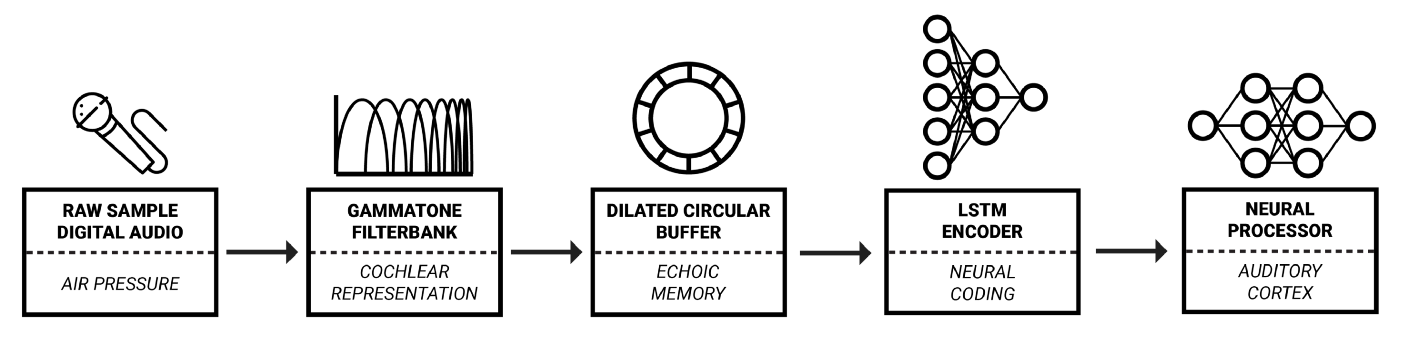
\includegraphics[width=1.0\textwidth]{Rothmann_Flow.png}  
	\caption{Rothmann's	\cite{rothmann} ML model of human hearing}
	\label{fig:rothman_flow}
\end{figure}

\begin{figure}[]
	\centering
	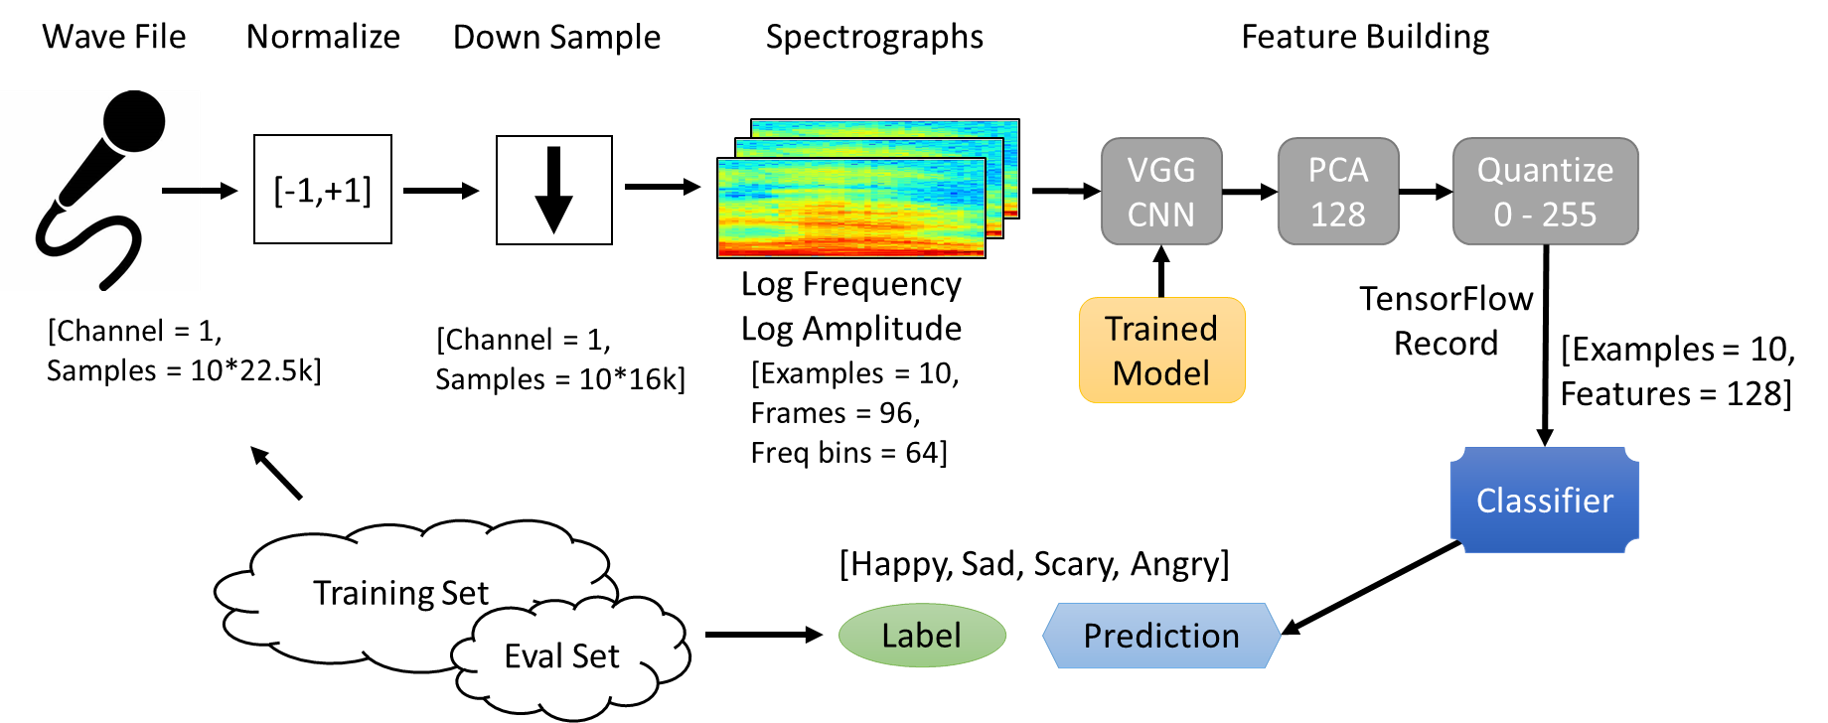
\includegraphics[width=1.0\textwidth]{VGG Flow.png}  
	\caption{Hershey \cite{hershey} model of converting \texttt{.wav} audio to features suitable for ML}
	\label{fig:vgg_flow}
\end{figure}
	
\section{Practical Implementation}

\subsection{Data Acquisition and Extraction}

We collected our data from Google’s AudioSet \cite{audioset} which consists of an expanding ontology of 632 audio event classes and a collection of 2,084,320 human-labeled 10-second sound clips drawn from YouTube videos. The ontology is specified as a hierarchical graph of event categories, covering a wide range of human and animal sounds, musical instruments and genres, and common everyday environmental sounds. From the dataset, we focused on music mood samples and extracted data instances having labels of four mood classes- \textit{Happy}, \textit{Sad}, \textit{Angry}, and \textit{Scary}. The dataset selected was divided into two groups: training and evaluation. 

To form our data sets, filtered from the ontology two sets: First, a set of 400 instances with our corresponding labels for training. Of these 400, we ensured we chose 100 entries of each mood classification. The second set contained 223 data points with ~56 instances per label which we used for evaluating our models. To avoid contamination, these 223 data instances were held aside during training and not introduced to the model until the evaluation stage. We created \texttt{.csv} files containing, for each instance, the YouTube video ID, start and stop times within the video, and the label associated with the instance. These \texttt{.csv}s were then used to run a batch processing script to download the audio samples in \texttt{.wav} format directly from their source (YouTube).

\subsection{Transformation to Features}
The next step in the application’s pipeline is to transform the raw \texttt{.wav} files into features that can be input into a classifier network. This is done via the process described above in section \ref{sec:theory}, using an open source TensorFlow model called VGGish \cite{vggish}. We made initial attempts to implement this layer ourselves, but the training required for the CNN to achieve suitable results is beyond the computational capacity of our local workstations. In this instance, to ‘see further, we stood on the shoulders of giants\cite{newton}’ (in this case, Google) and used the pre-trained CNN model to feature-ize the \texttt{.wav} files. We converted each of our 400+223 \texttt{.wav} file instances using VGGish to 128x10 element feature vectors.

\subsection{Classification}

After initial processing of the wav files into feature vectors (matrices) of dimension 128x10 we investigated different models to perform the multi-class classification task of predicting the ‘mood’ of the music from the feature vector.

To evaluate different classification models, Python was used enlisting the libraries TensorFlow\cite{tensorflow} and Keras\cite{keras}.

The 400 training samples were evenly divided by class for stratified cross validation and used to train 3 different neural networks:
\begin{enumerate}
\item Simple multi-class logistic regression classifier
\item 1-Layer LSTM (Long-short term memory) recurrent neural network
\item 3-Layer LSTM (Long-short term memory) recurrent neural network
\end{enumerate}
In each case, the model was trained using batches of 40 samples, randomized at each presentation, for a sufficient number of epochs to infer steady-state accuracy.

We evaluated the performance of each of the 3 models by two methods:
\begin{enumerate}
\item Validation set accuracy over an increasing number of epochs, to watch for over-training and the any generalization gap.
\item Evaluation on a Test Set of 220 never-seen-before data instances.
\end{enumerate}

The performance of the training sessions is shown in figure \ref{fig:baseline_train}.
\begin{figure}[]
	\centering
	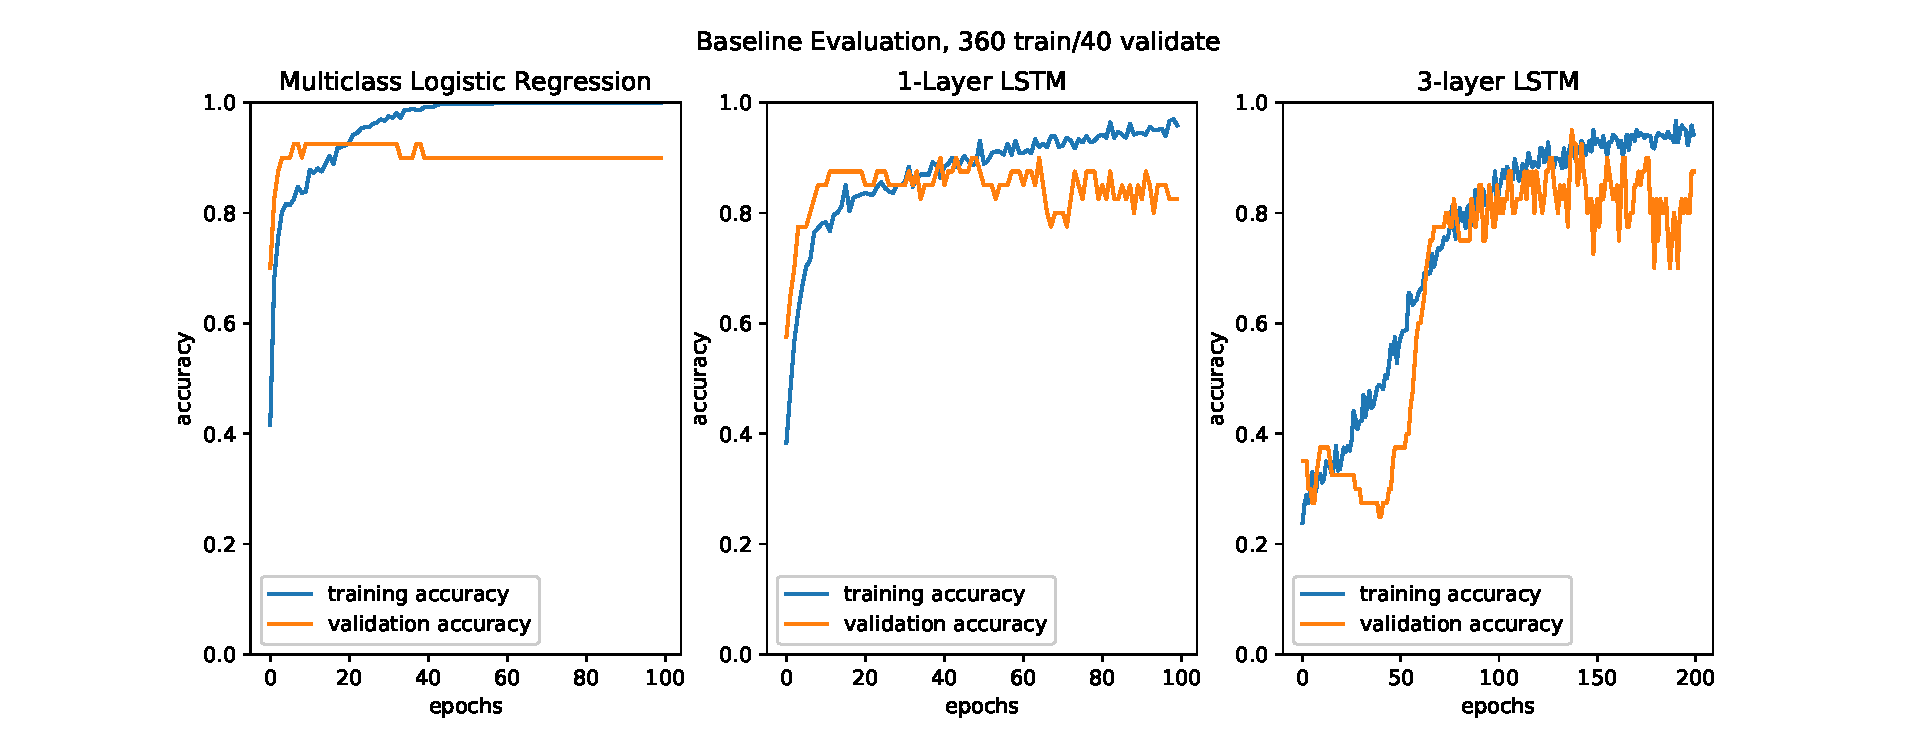
\includegraphics[width=1.25\textwidth]{Baseline400.eps}  
	\caption{Baseline training performance for 3 models.}
	\label{fig:baseline_train}
\end{figure}

After training, the evaluation on  the 220-instance balanced test set, we observed the accuracies shown in table \ref{tbl:baseline_acc}.
\begin{table}[] 
\caption{Baseline accuracy on held-aside test set of 220 instances for 3 models.}
\label{tbl:baseline_acc}
\centering
\begin{tabular}{lc} 
\toprule
\hline
Model & Accuracy \\ 
\midrule
Logistic Regression & 0.803 \\
1-Layer LSTM & 0.830 \\ 
3-Layer LSTM & 0.731 \\ 
\bottomrule
\end{tabular}
\end{table}

Finally, to make sure that our four chosen classes do not have an abnormal correlation between any combinations of classes, we also computed confusion matrices for the models. The confusion matrix for Logistic Regression (arguably the best performing classifier) is shown in table \ref{tbl:baseline_conf}.

\begin{table}[] 
\caption{Confusion matrix for baseline logistic regression classifier of 223 test instances.}
\label{tbl:baseline_conf}
\centering
\begin{tabular}{lcccc} 
\toprule
\hline
 & Happy & Sad & Angry & Scary \\ 
\midrule
Happy & 45 &  9 & 2 & 1 \\
Sad   &  11 & 39 & 2 & 4 \\
Angry &  0 &  1 & 53 & 4 \\
Scary &  0 &  7 & 3 &  42 \\
\bottomrule
\end{tabular}
\end{table}

From the baseline evaluation we can draw some conclusions and inferences:
\begin{itemize}
\item The input feature sets must be nearly linearly separable, as evidenced by the strong performance of the simple multiclass logistic regression classifier.
\item Google’s preprocessing of the raw audio waveforms into 10-frame spectrographs, including processing by Google’s own CNN and PCA reduction clearly has produced data that is well separated without significant further processing.
\item Evidence of the linearly separable feature data is supported by much more complicated non-linear classifiers (1-Layer LSTM and 3-Layer LSTM) not yielding better performance.
\item There is evidence that the LSTM models are subject to overtraining at higher numbers of epochs.
\item More complicated models with more parameters, particularly the 3-Layer LSTM, take significantly more time to train.
\item The confusion matrix suggests, surprisingly, that ‘Happy’ and ‘Sad’ are the most often confused classifications, and that ‘Scary’ and ‘Angry’ are comparatively easy to predict.
\end{itemize}


\section{Conclusion}

\subsection{Discussion}

\subsection{Future Work}
  
\bibliography{Bibliography} 
\bibliographystyle{plainnat}

\end{document}
